

%%%%%%%%%%%%%%%%%%%%%%%%%%%%%%%%%%%%%%%%%%%%%%%%%%%%%%%%%%%%%%%%%%%%%%%%%%%%%%%%%%%
%%                 PŘÍLOHA - UŽIVATELSKÁ PŘÍRUČKA                                %%
%%%%%%%%%%%%%%%%%%%%%%%%%%%%%%%%%%%%%%%%%%%%%%%%%%%%%%%%%%%%%%%%%%%%%%%%%%%%%%%%%%%
\chapter{User guide}
\label{user-guide}

This user guide is written for plugin using in QGIS 2.12. There is a~possibility that works with plugin
will be different in other versions of QGIS. 

\section{Loading of plugin}
\label{plugin-load}

* 
* 

* 
* TUHLE ČÁST JEŠTĚ MUSÍM DOPSAT - NEJDŘÍV JE POTŘEBA PLUGIN ZE SLOŽKY SUROLEVELING FUNKČNĚ PŘESUNOUT DO GPS POSITION LAG CORRECTION, ABYCH VĚDĚL, JAK SE BUDE V NABÍDCE PLUGIN JMENOVAT
*

* 
*

\section{Work with plugin}
\label{work}

In this section will be described primary functions and working of graphical user interface of plugin. 

  \begin{figure}[H]
   \centering
	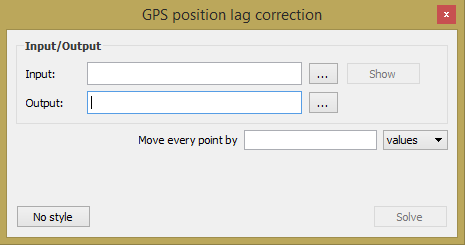
\includegraphics[scale=0.75]{./pictures/gui.png}
	\caption[GUI]{GUI}
      \label{fig:gui}
  \end{figure}

\subsection{Input and output defining}
\label{input-output}

The basic elements are of course input and output. 

In input, you have to define the~file you want to work with. You can write the~path to this file or
there is the~button with {\tt ...}. If you click on this button, you will get the~interface where
you can choose the~path to your file. Click on OK will insert this path to lineedit in basic GUI. Click
on Cancel will interrupt the~interface for choose, and the~content of lineedit will not be changed. 

  \begin{figure}[H]
   \centering
	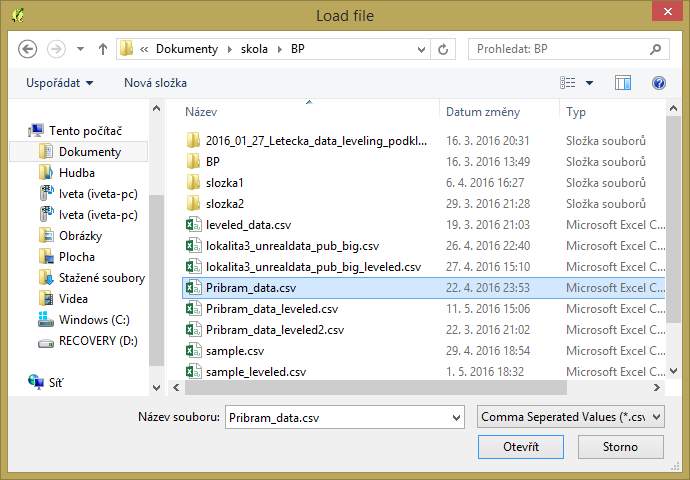
\includegraphics[scale=0.75]{./pictures/input.png}
	\caption[Loading input]{Loading input}
      \label{fig:input}
  \end{figure}

The~same work is with output, but there you define the~path where the~new file will be created.
You can manually define the~path or use the~browse button. You will again get a~new interface, this
time created for choosing folder. 

  \begin{figure}[H]
   \centering
	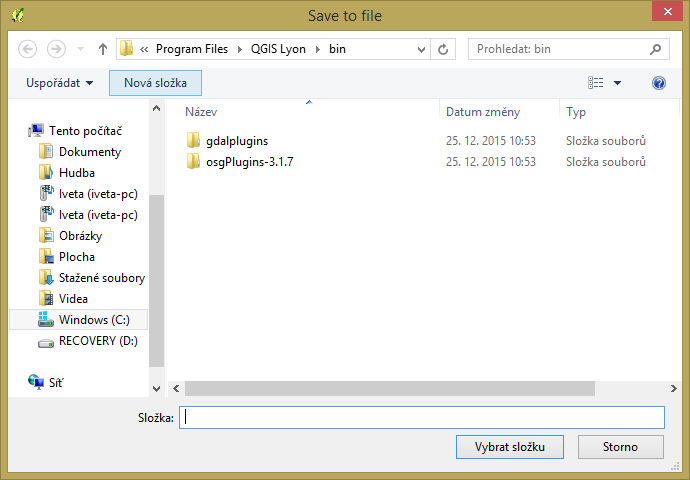
\includegraphics[scale=0.75]{./pictures/output.png}
	\caption[Choosing output directory]{Choosing output directory}
      \label{fig:output}
  \end{figure}

\subsection{Styling}
\label{styling}

There is also additional possibility of styling your points for better visualisation. 

In the~default GUI is the~button \textit{No style}. It means that you have not defined any style
and points will be created in default QGIS style. If you want your own style, you have to click on
this button. You will get the~browsing interface. You are automatically directed to folder
\textit{styles} in the~plugin folder; you have to choose qml file and click OK. Click on Cancel will
interrupt the interface and set again \textit{No style}. 

  \begin{figure}[H]
   \centering
	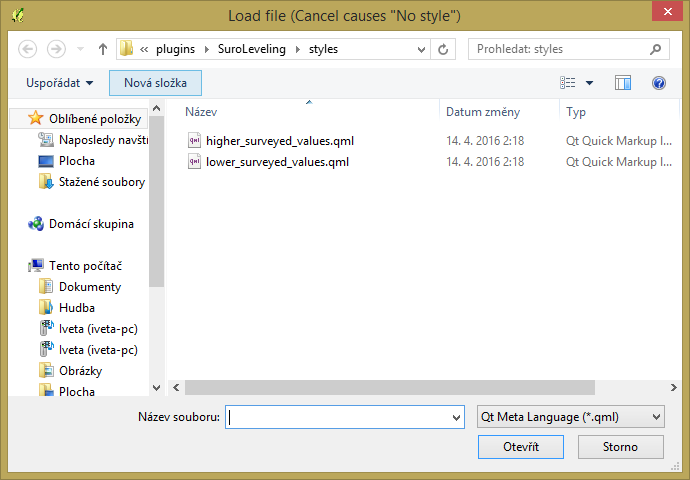
\includegraphics[scale=0.75]{./pictures/style.png}
	\caption[Choose style]{Choose style}
      \label{fig:style}
  \end{figure}

If you have chosen your own style, you would see its name on the~style button. 

  \begin{figure}[H]
   \centering
	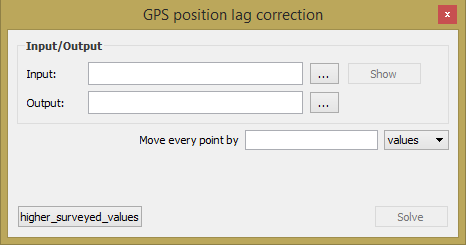
\includegraphics[scale=0.75]{./pictures/style-defined.png}
	\caption[Used style]{Used style}
      \label{fig:used-style}
  \end{figure}

In the~default version of plugin there are two default styles. Styling in those styles is based on
column mereni – one style for higher and one style for lower values. 

\subsection{Showing input}
\label{show}

Next to input is the button \textit{Show}. 

Show button is just to visualise the input file as layer in QGIS. It has no effect on the run of plugin
and it is not necessary for the~run, but it allows you to visualise the~input file in the same style as
the~output file. It gives you also the~opportunity to compare the~moved values with the~original ones. 

This button was created on request by users who prefer to visualise both the~input and the~output in
the~same interface. 

If input file does not exists, plugin will raise the~error message. 

\subsection{Move}
\label{move}

Move will be done by clicking on button \textit{Solve}. Before moving you have to define few more things. 

In combobox you can choose the~units of move – each presents other type of move; values mean move
by values, meters mean move by constant distance and seconds mean move by constant time/variable
distance considering current velocity. 

In the~appropriate lineedit you have to insert value of move. For values it should be integer (it
does not make sense to move point by 1.5 values because nothing like 1.5 value does not exist), for
other moves it should be integer or float. 

For wrong input, plugin will raise the~error message. 

\subsection{Dependencies}
\label{dependencies}

To avoid some unnecessary errors, there are some dependencies in the~plugin GUI. 

The~first is \textit{Show} button. This button is
disabled until you have wrote anything into input lineedit. 

  \begin{figure}[H]
   \centering
	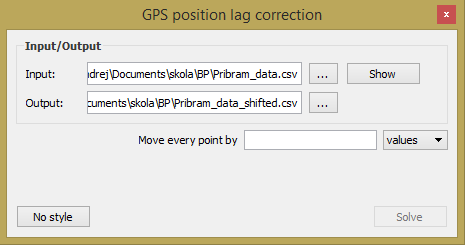
\includegraphics[scale=0.75]{./pictures/show.png}
	\caption[Enabled Show button]{Enabled Show button}
      \label{fig:show}
  \end{figure}

The~second is button \textit{Solve}. You can’t solve anything until you have defined input, output and
value of move.

  \begin{figure}[H]
   \centering
	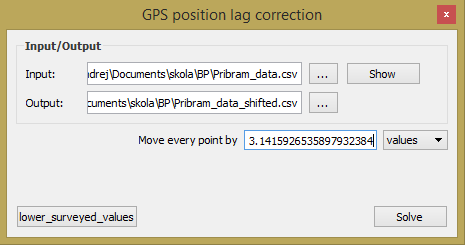
\includegraphics[scale=0.75]{./pictures/solve.png}
	\caption[Enabled Solve button]{Enabled Solve button}
      \label{fig:solve}
  \end{figure}

There is also implemented shortcut for defining output directory. Many users wants to save output file to
the~directory from which was read the~input file, so when you choose input file, the~directory will
be automatically copied into output lineedit, just with added \textit{\_moved} into filename. 
